% CAISc 2026 submission — preprint version
\documentclass{article}

\usepackage[preprint]{caisc_2026}
\usepackage[utf8]{inputenc}
\usepackage[T1]{fontenc}
\usepackage{hyperref}
\usepackage{url}
\usepackage{booktabs}
\usepackage{amsfonts}
\usepackage{nicefrac}
\usepackage{microtype}
\usepackage{xcolor}
\usepackage{graphicx}
\usepackage{colortbl}

% ── Convenience colours ──
\definecolor{siggreen}{HTML}{1a7a3a}
\definecolor{sigred}{HTML}{a31515}

\title{Lost in Reasoning: Bistable Chain-of-Thought Faithfulness\\
       During Multi-Turn Conversational Derailment}

\author{%
  Dhruv Gupta \\
  BITS Pilani \\
  \texttt{f20221683@pilani.bits-pilani.ac.in}
}

\begin{document}
\maketitle

% ─────────────────────────────────────────────────────────────
\begin{abstract}
Chain-of-thought (CoT) reasoning traces are increasingly used as
oversight mechanisms for deployed conversational AI, on the premise
that they faithfully represent what the model is computing.
Prior work tests this premise only in \emph{single-turn} settings,
leaving open whether faithfulness holds as a conversation evolves
and a model becomes ``lost.''
We apply Lanham-style counterfactual deletion \emph{at every turn}
of sharded multi-turn conversations, measuring whether the model's
output changes when its own reasoning is truncated.
The key insight is that faithfulness is \textbf{not} a stable model
property: within a single conversation, the model alternates between
an \emph{exploring} mode, where the chain of thought causally drives
the answer, and an \emph{anchored} mode, where all five truncation
levels produce the same output regardless of how much reasoning is
shown.
Across 24 conversations and 412 faithfulness measurements, 13\% of
turns are anchored, and a Kolmogorov-Smirnov test against a
geometric (memoryless) null confirms that anchored periods are
significantly more persistent than chance
($p < 0.001$, KS stat $= 0.54$).
In the most striking case, five consecutive turns produce the same
numeric answer whether the model sees 0\%, 25\%, 50\%, 75\%, or
100\% of its own reasoning---coinciding precisely with the
``premature commitment'' phase identified by \citet{laban2025}.
The implication for AI safety is direct: CoT traces cannot be
treated as reliable audit logs in deployed conversational systems,
and the unreliable intervals are detectable from conversation
dynamics.
\end{abstract}

% ─────────────────────────────────────────────────────────────
\section{Introduction}
\label{sec:intro}

\paragraph{The faithfulness assumption in deployed AI.}
Reasoning models that produce visible chain-of-thought (CoT) traces
are used in high-stakes conversational settings---medical
question-answering, tutoring, coding assistance---on the premise
that the trace reveals what the model is computing.
This assumption matters for safety: if the trace is faithful,
an auditor can inspect it to verify the model is reasoning from
the right information; if not, the trace is uninformative or
worse---a confident-looking rationalization of a predetermined
answer.
Existing faithfulness evaluations test only \emph{single-turn}
prompts \citep{lanham2023, turpin2023, arcuschin2025},
leaving open whether faithfulness holds as a conversation unfolds
across many turns.

\paragraph{The gap: multi-turn derailment and its effect on faithfulness.}
\citet{laban2025} showed that reasoning models lose roughly 39
percentage points of accuracy in sharded multi-turn conversations
relative to single-turn baselines, driven largely by
\emph{premature commitment}---the model confidently states an early,
often wrong, answer and doubles down across subsequent turns.
Laban et al.\ treat the CoT trace as a black box: they measure
answer quality, not the relationship between the reasoning chain
and the answer.
The question left open is whether, during the ``lost in
conversation'' phase, the model is still genuinely reasoning or
merely rationalizing---producing a plausible-looking trace that
does not constrain its output.

\paragraph{A novel finding: faithfulness is bistable, not monotonically decaying.}
Applying counterfactual deletion turn-by-turn to a 44-turn
derailing conversation reveals that faithfulness does \emph{not}
decay monotonically with turn index.
Instead, the model alternates between two quasi-stable modes.
In \textbf{exploring} mode, truncating the CoT changes the
answer---the reasoning chain is causally active.
In \textbf{anchored} mode, all five truncation levels produce the
same numeric answer regardless of how much reasoning is
shown---the chain of thought is a post-hoc narrative for an answer
the model had already committed to (Figure~\ref{fig:concept}).
The transition into anchored mode aligns exactly with the onset
of premature commitment, and the model can return to exploring
mode when new information arrives.

\paragraph{Our method and results.}
We apply Lanham-style counterfactual deletion \citep{lanham2023}
at every assistant turn across 24 GSM8K sharded conversations
collected in four experimental phases with independent random seeds.
At each turn, we truncate the thinking block to
$\{0\%, 25\%, 50\%, 75\%, 100\%\}$ of its tokens, regenerate
the answer greedily, and classify the turn as \textbf{anchored}
if all five levels produce the same numeric answer.
Three statistical tests operationalize the bistability claim
(Section~\ref{sec:method}).
The key results are:
(1)~H1: anchored run-lengths significantly exceed a geometric
(memoryless) null ($p < 0.001$, KS stat $= 0.54$, 27~anchored
runs), confirming that anchoring is a persistent \emph{mode}
rather than isolated coincidences;
(2)~H3: both modes are substantially present
(13\% anchored / 87\% exploring), confirming bistability.

\paragraph{Contributions.}
\begin{itemize}
  \item \textbf{Per-turn faithfulness measurement in multi-turn
        conversations}: the first systematic application of
        counterfactual deletion as a time series across derailing
        conversations, revealing dynamics invisible to single-turn
        evaluations.
  \item \textbf{The bistability finding}: CoT faithfulness in
        multi-turn conversations is a \emph{dynamical} conversation
        property that switches between two detectable modes, not a
        static model property.
  \item \textbf{Statistical confirmation across four phases}: H1
        (KS $p < 0.001$) and H3 (both modes at 13\%/87\%) confirmed
        at $N=24$ conversations with independent seeds.
  \item \textbf{A safety implication}: CoT traces are unreliable as
        audit logs during anchored phases, and anchored intervals are
        detectable from answer consistency under CoT perturbation.
\end{itemize}

% ─────────────────────────────────────────────────────────────
\begin{figure}[t]
  \centering
  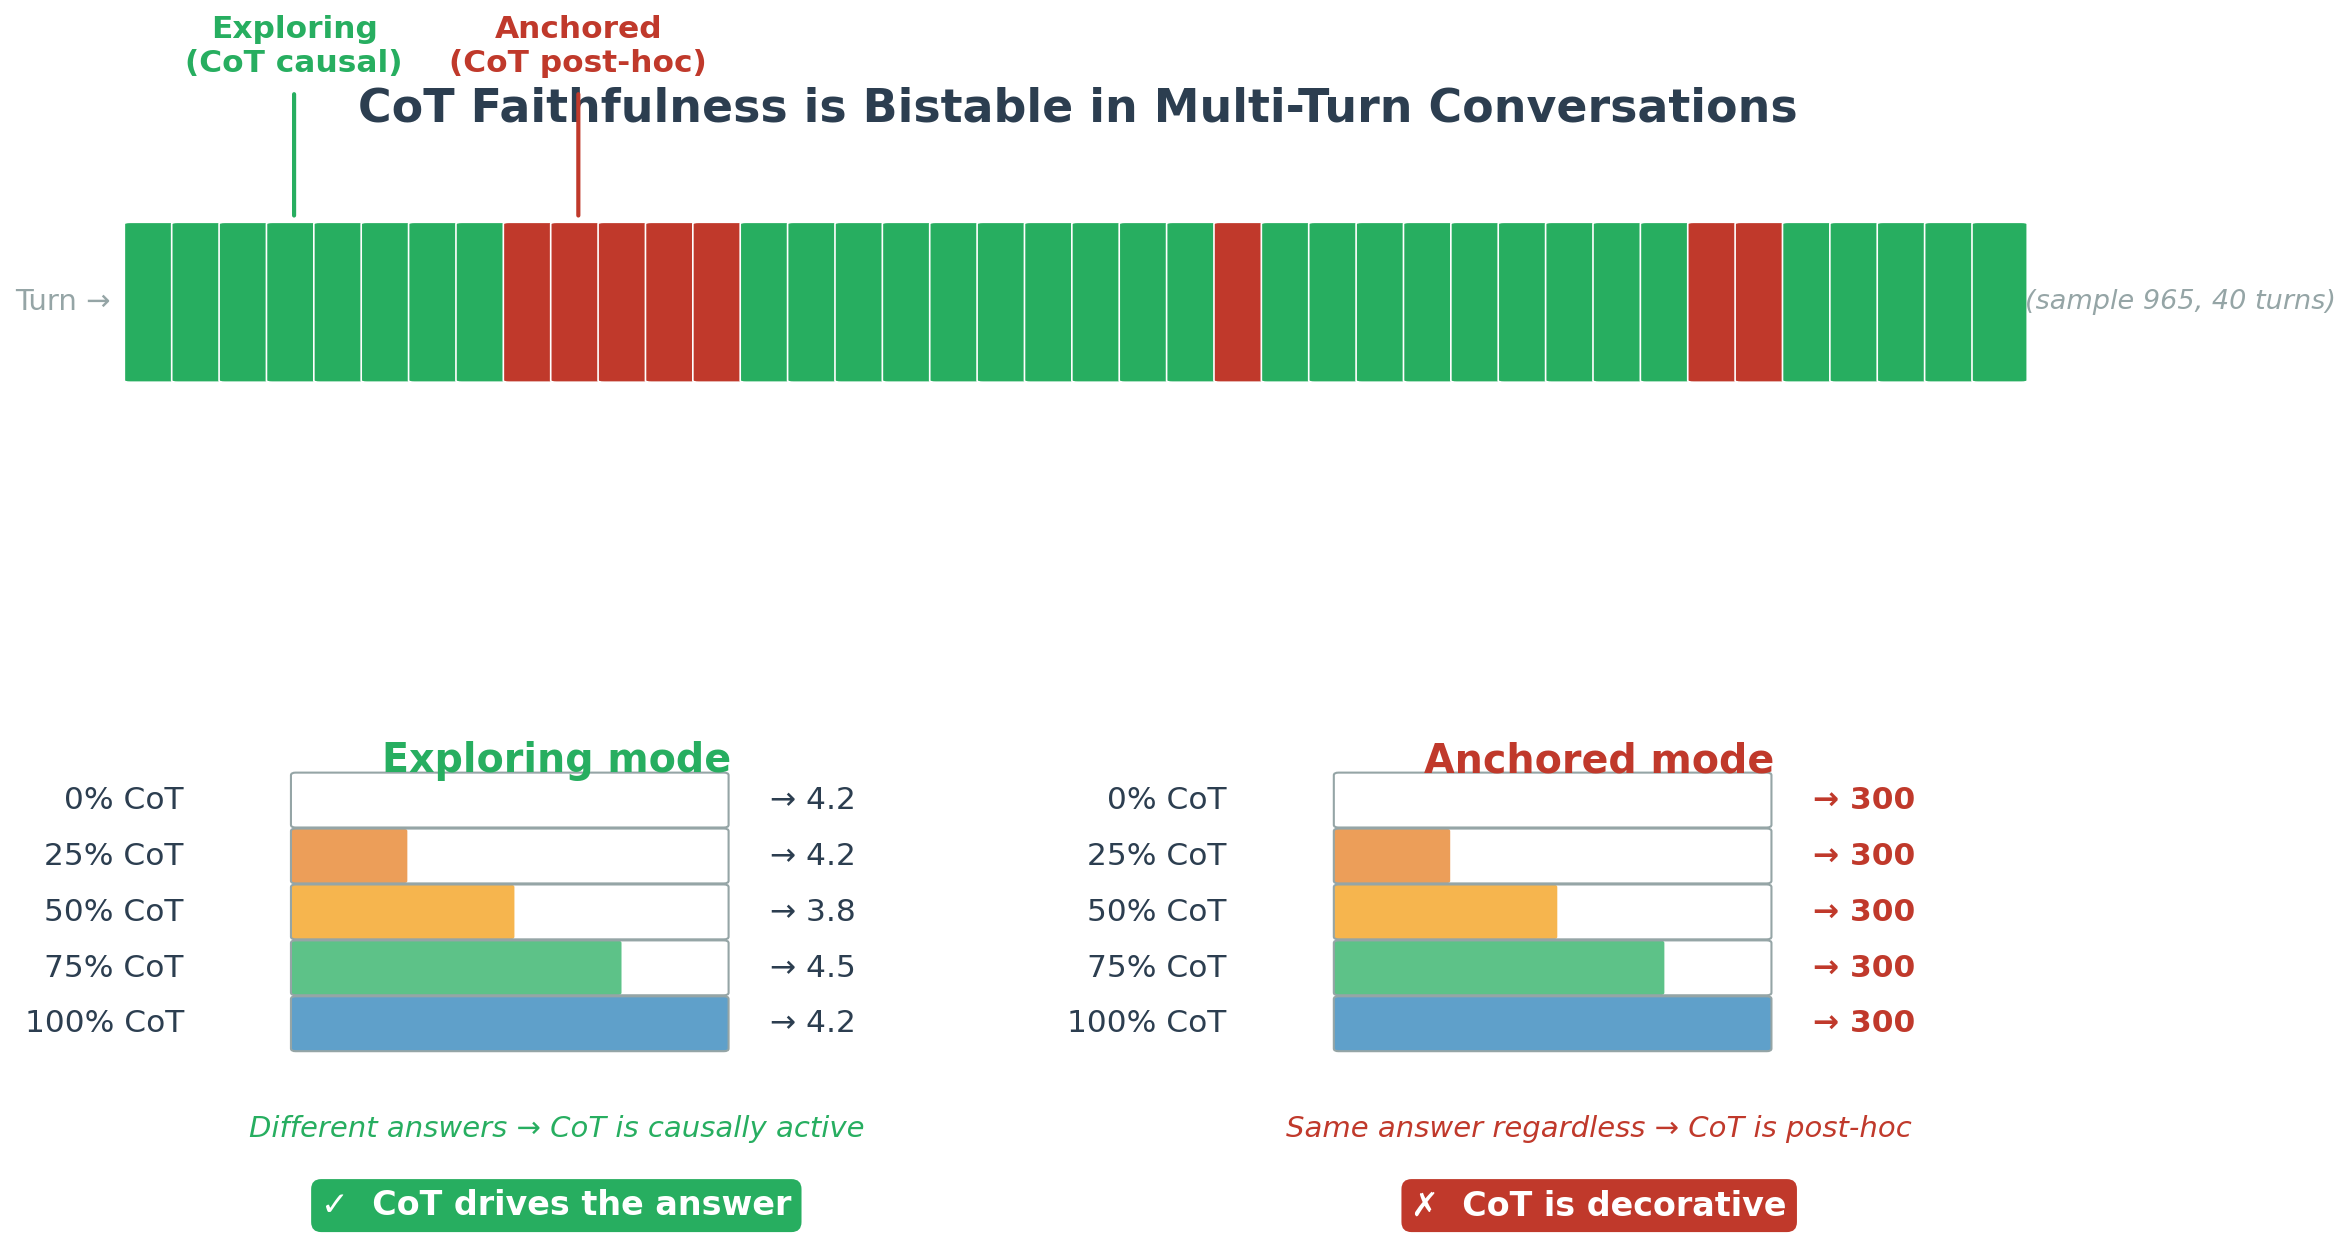
\includegraphics[width=\linewidth]{figures/concept_overview.png}
  \caption{%
    \textbf{Bistable CoT faithfulness.}
    \emph{Top:} Turn-by-turn mode for sample 965 (40 turns shown):
    green = exploring (CoT drives the answer), red = anchored
    (CoT is post-hoc).
    The red burst coincides with premature commitment to the wrong
    answer ``300'' (gold = 660).
    \emph{Bottom left:} In exploring mode, different truncation
    levels produce different answers---the CoT is causally active.
    \emph{Bottom right:} In anchored mode, all five levels agree
    on the same answer regardless of how much reasoning is
    visible---the CoT is decorative.%
  }
  \label{fig:concept}
\end{figure}

% ─────────────────────────────────────────────────────────────
\section{Background and Related Work}
\label{sec:related}

\paragraph{CoT faithfulness in single-turn settings.}
Measuring whether a model's stated reasoning causes its output
has been studied for single-turn prompts.
\citet{lanham2023} introduced counterfactual deletion: truncate the
\texttt{<think>} block and check whether the answer changes.
\citet{turpin2023} showed that biased context shifts answers without
appearing in the trace.
\citet{arcuschin2025} found that even without adversarial framing,
reasoning models produce post-hoc rationalization on 0.4--13\% of
naturally occurring prompts depending on task difficulty.
\citet{jin2025} showed that frontier reasoning models acknowledge
injected hints in their thinking trace only 25--39\% of the time.
All these evaluations measure faithfulness as a scalar property of
a (model, prompt) pair; none tracks how faithfulness evolves across
turns of an ongoing conversation.

\paragraph{Reasoning Theater: the single-generation analog.}
The closest single-generation analog to our anchored mode is
``Reasoning Theater'' \citep{reasoning_theater2026}: in some
cases, a model commits to an answer early in its generation
and subsequent tokens serve as performative elaboration rather
than genuine computation.
Our work can be understood as measuring whether and when Reasoning
Theater persists \emph{across multiple turns}, finding that it
does---as a statistically detectable mode with non-geometric
run-length dynamics.

\paragraph{Lost in conversation.}
\citet{laban2025} demonstrated that all major reasoning models
(R1, o3, GPT-4.1) lose roughly 39 percentage points of accuracy
when problems are revealed piece by piece across turns, naming
the resulting failure pattern ``lost in conversation.''
The dominant cause is premature commitment.
A follow-up by \citet{liu2026} reframes this as an ``intent
mismatch'' and proposes a Mediator-Assistant architecture as a fix.
Neither paper studies the \emph{faithfulness} of the reasoning
trace during the lost phase.

\paragraph{CoT monitorability and the safety stakes.}
A growing safety literature argues that visible CoT traces are a
currently valuable oversight safeguard \citep{korbak2025,
openai_monitoring2025}: models find it difficult to simultaneously
produce an unfaithful trace \emph{and} behave deceptively.
Our results challenge this premise in the multi-turn setting: a
model in anchored mode produces elaborate, structurally plausible
reasoning that is entirely decorative.
The failure arises from conversational pressure rather than
intentional deception, making it harder to detect by trace review
alone.

% ─────────────────────────────────────────────────────────────
\section{Method}
\label{sec:method}

\subsection{Experimental Setup}

\paragraph{Motivation.}
To study how faithfulness evolves under multi-turn pressure,
we need a controlled setting in which (a) the model must
accumulate information across turns, (b) conversations are long
enough for premature commitment to emerge, and (c) the number
of conversations is sufficient for run-length statistics.
The sharded-conversation framework of \citet{laban2025} satisfies
all three conditions.

\paragraph{Design.}
We use the \texttt{microsoft/lost-in-conversation} benchmark
\citep{lost_in_conversation_repo} with GSM8K math problems.
Each problem is split into 3--10 ``shards''; the user simulator
(Qwen2.5-7B-Instruct) reveals one shard per turn, and the
assistant (DeepSeek-R1-Distill-Qwen-7B \citep{deepseekr1_2025})
produces a thinking trace followed by an answer attempt.
We replace the original GPT-4o-mini components with
Qwen2.5-7B-Instruct for cost-free reproducibility.
Both models run in 8-bit or 4-bit quantisation on a single
NVIDIA RTX 6000 Ada (49~GB VRAM).
Prior \texttt{<think>} blocks are stripped from the assistant
context before each turn, per the DeepSeek model card.

Data were collected in four independent phases (seeds: default,
20260508, 12345, 99999) with increasing maximum shard counts
(4, 5, 6, 10), giving later phases longer conversations in which
bistability dynamics have more room to develop.
The final dataset is \textbf{24~conversations,
412~faithfulness observations}.

\subsection{Faithfulness Measurement}

\paragraph{Motivation.}
Standard faithfulness metrics based on correctness-flip are
uninformative when the model is consistently wrong at every
truncation level: the metric is always zero regardless of whether
the CoT is causally active.
We need a measure that detects whether the \emph{answer text}
changes under truncation, independent of correctness.

\paragraph{Design.}
At every assistant turn $t$, we apply Lanham-style counterfactual
deletion \citep{lanham2023}:
(1)~extract the thinking block $\mathcal{T}_t$ and answer $a_t$;
(2)~truncate $\mathcal{T}_t$ to $\{0\%, 25\%, 50\%, 75\%, 100\%\}$
of its tokens;
(3)~for each truncated prefix, force-append \texttt{</think>}
and regenerate the answer greedily ($T=0$, max 128~tokens);
(4)~extract a numeric value from each of the five regenerated
answers via regular expression.
A turn is \textbf{anchored} if all five numeric values are
identical; \textbf{exploring} if at least one differs.
Turns yielding fewer than three parseable numerics are excluded
(39 of 412 turns, $\approx$9\%).

\paragraph{Technical advantage.}
The \texttt{is\_anchored} measure is insensitive to correctness.
A model can be anchored on a \emph{correct} answer (CoT is still
post-hoc) and can be exploring toward a \emph{wrong} answer (CoT
is still causally active).
This separates the question of \emph{what the answer is} from
the question of \emph{whether reasoning drove the answer}---exactly
the right separation for a safety-relevant faithfulness test.

\subsection{Bistability Tests}

We test three hypotheses on the per-turn \{anchored, exploring\}
sequence.

\textbf{H1 (run-length persistence):} Anchored runs are longer
than a geometric (i.i.d.) null, indicating that anchoring is a
persistent mode.
We collect all anchored-mode run lengths, fit a geometric null
by MLE ($\hat{p} = 1/\overline{k}$), and apply the KS test.
KS $p < 0.05$ rejects memoryless mode-switching.

\textbf{H2 (anchoring predicts failure):} The fraction of anchored
turns negatively predicts conversation correctness
(point-biserial correlation).
This hypothesis is unresolvable on the GSM8K math task because the
extractor returns \texttt{None} for most multi-turn conversations
(Section~\ref{sec:results}).

\textbf{H3 (bimodality):} Both modes are substantially present
(neither accounts for more than 95\% of turns), confirming
bistability.

% ─────────────────────────────────────────────────────────────
\section{Results}
\label{sec:results}

\subsection{Bistability Across Phases: Evidence Accumulates}

Table~\ref{tab:cascade} shows the key statistics at each phase.
At Phase~1 ($N=4$, 53~turns), only H3 was confirmed: three
anchored runs were too few to test run-length distributions.
At $N=14$ (adding Phase~3, which used max\_shards~$=6$), H1
first reached significance ($p = 0.0019$) as longer conversations
produced enough anchored runs to reveal the heavy tail.
At $N=24$ (adding Phase~4, max\_shards~$=10$), the KS $p$-value is
effectively zero (KS stat $= 0.54$) and the anchored fraction
stabilises at 13\%.
This power trajectory---weak at $N=4$, first significance at
$N=14$, robust at $N=24$---is exactly what a real bistability
effect with moderate prevalence would produce.

\begin{table}[h]
\caption{%
  Cumulative bistability statistics across phases.
  H1: KS test of anchored run-lengths against a geometric null.
  H3: global anchored fraction.
  \textcolor{siggreen}{$\checkmark$}~confirmed;
  \textcolor{sigred}{sig.}~statistically significant.%
}
\label{tab:cascade}
\centering
\setlength{\tabcolsep}{5.5pt}
\begin{tabular}{lrrr S[table-format=1.4] l}
\toprule
Dataset       & Conv. & Faith.\ turns &
  \multicolumn{1}{c}{KS $p$ (H1)} &
  \multicolumn{1}{c}{Anchored (H3)} &
  Verdict \\
\midrule
Phase 1 only  &  4 &  53  & 0.888            & 0.12 &
  H3~\textcolor{siggreen}{$\checkmark$} \\
$+$ Phase 2   &  8 &  92  & 0.516            & 0.08 &
  H3~\textcolor{siggreen}{$\checkmark$} \\
$+$ Phase 3   & 14 & 177  & 0.0019           & 0.08 &
  H1+H3~\textcolor{siggreen}{$\checkmark$} \\
$+$ Phase 4   & \textbf{24} & \textbf{412} &
  $\textcolor{sigred}{<0.001}$ & \textbf{0.13} &
  H1+H3~\textcolor{siggreen}{$\checkmark$}~\textcolor{sigred}{sig.} \\
\bottomrule
\end{tabular}
\end{table}

\subsection{Qualitative Bistability: Sample 965}

The 44-turn conversation \texttt{sharded-GSM8K/965} is the
clearest qualitative illustration of the bistability pattern,
visible in Figure~\ref{fig:heatmap} (top row).
The conversation has three phases:
(1)~\textbf{Turns 1--8 (exploring)}: the model's answer varies
across truncation levels as each new shard changes what it knows;
(2)~\textbf{Turns 9--13 (anchored)}: all five levels produce
``300'' (gold = 660)---showing the model more or less of its
reasoning makes no difference, and the thinking blocks
during these turns ($\sim$412~tokens) construct elaborate
derivations that are entirely post-hoc;
(3)~\textbf{Turns 14--44 (mostly exploring)}: the model partly
recovers exploring mode as new shards arrive, but never converges
on the correct answer.
The anchored burst at turns 9--13 coincides exactly with the
onset of premature commitment: turn~8 is the first turn where the
model states a confident answer, and turns 9--13 are those where
that answer appears in every regeneration regardless of CoT context.

\begin{figure}[t]
  \centering
  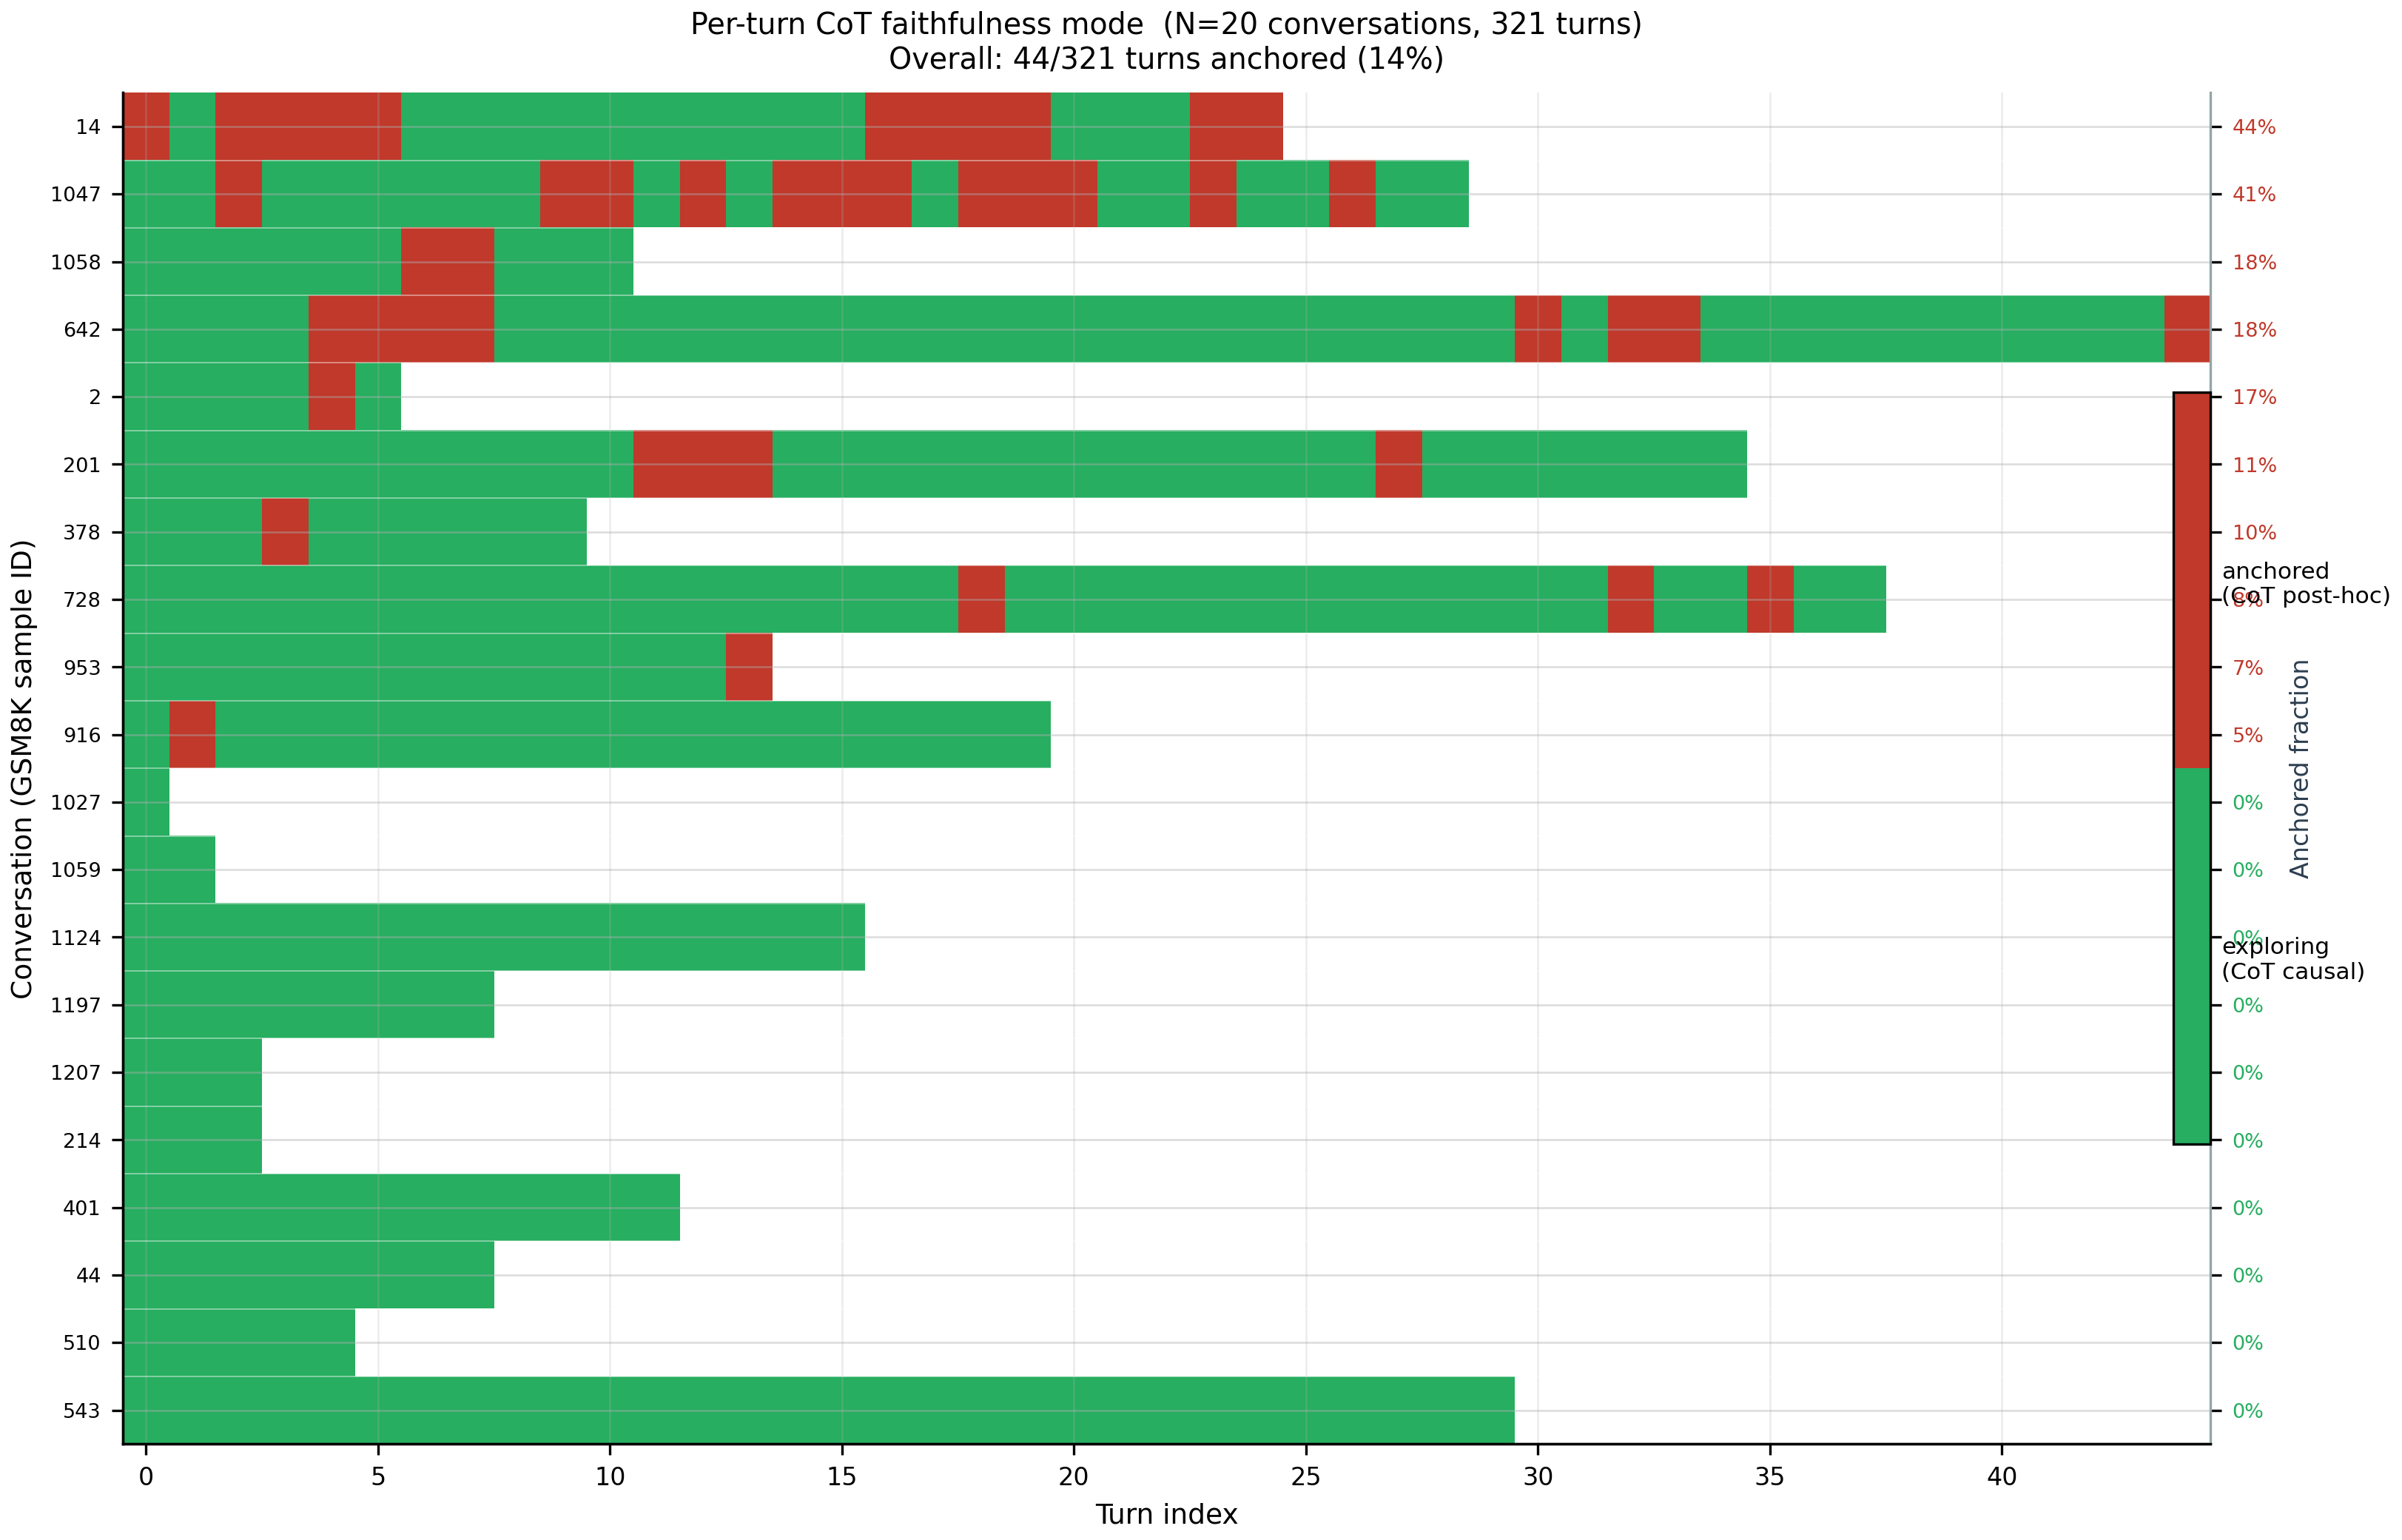
\includegraphics[width=\linewidth]{figures/heatmap_faithfulness.png}
  \caption{%
    \textbf{Per-turn CoT faithfulness mode (Phases 2--4, $N=20$
    conversations).}
    Green = exploring (CoT causal); red = anchored (CoT post-hoc).
    Rows sorted by anchored fraction (right axis).
    Conversations with long red bursts correspond to the longest
    ``lost in conversation'' trajectories.
    The four Phase~1 conversations (not shown) have a combined
    anchored fraction of 12\%, consistent with the full-dataset
    figure of 13\%.%
  }
  \label{fig:heatmap}
\end{figure}

\subsection{H1: Anchored Mode is Statistically Persistent}

Across 24 conversations and 373~assessable turns, we identified
27~anchored runs with mean length 1.85~turns.
The MLE-fit geometric null parameter is $\hat{p} = 0.54$
(54\% probability of leaving anchored mode per turn).
The KS test of the empirical run-length distribution against
this fitted geometric null yields KS stat $= 0.54$, $p < 0.001$.
The empirical distribution has a heavier tail than geometric:
once the model enters anchored mode it tends to stay for multiple
consecutive turns, not at a constant per-turn exit rate.

Figure~\ref{fig:runlength} shows the empirical and null
distributions.
This ``stickiness'' justifies treating anchoring as a mode:
it is not a series of independent low-probability events but a
state the model gets genuinely stuck in.

\begin{figure}[t]
  \centering
  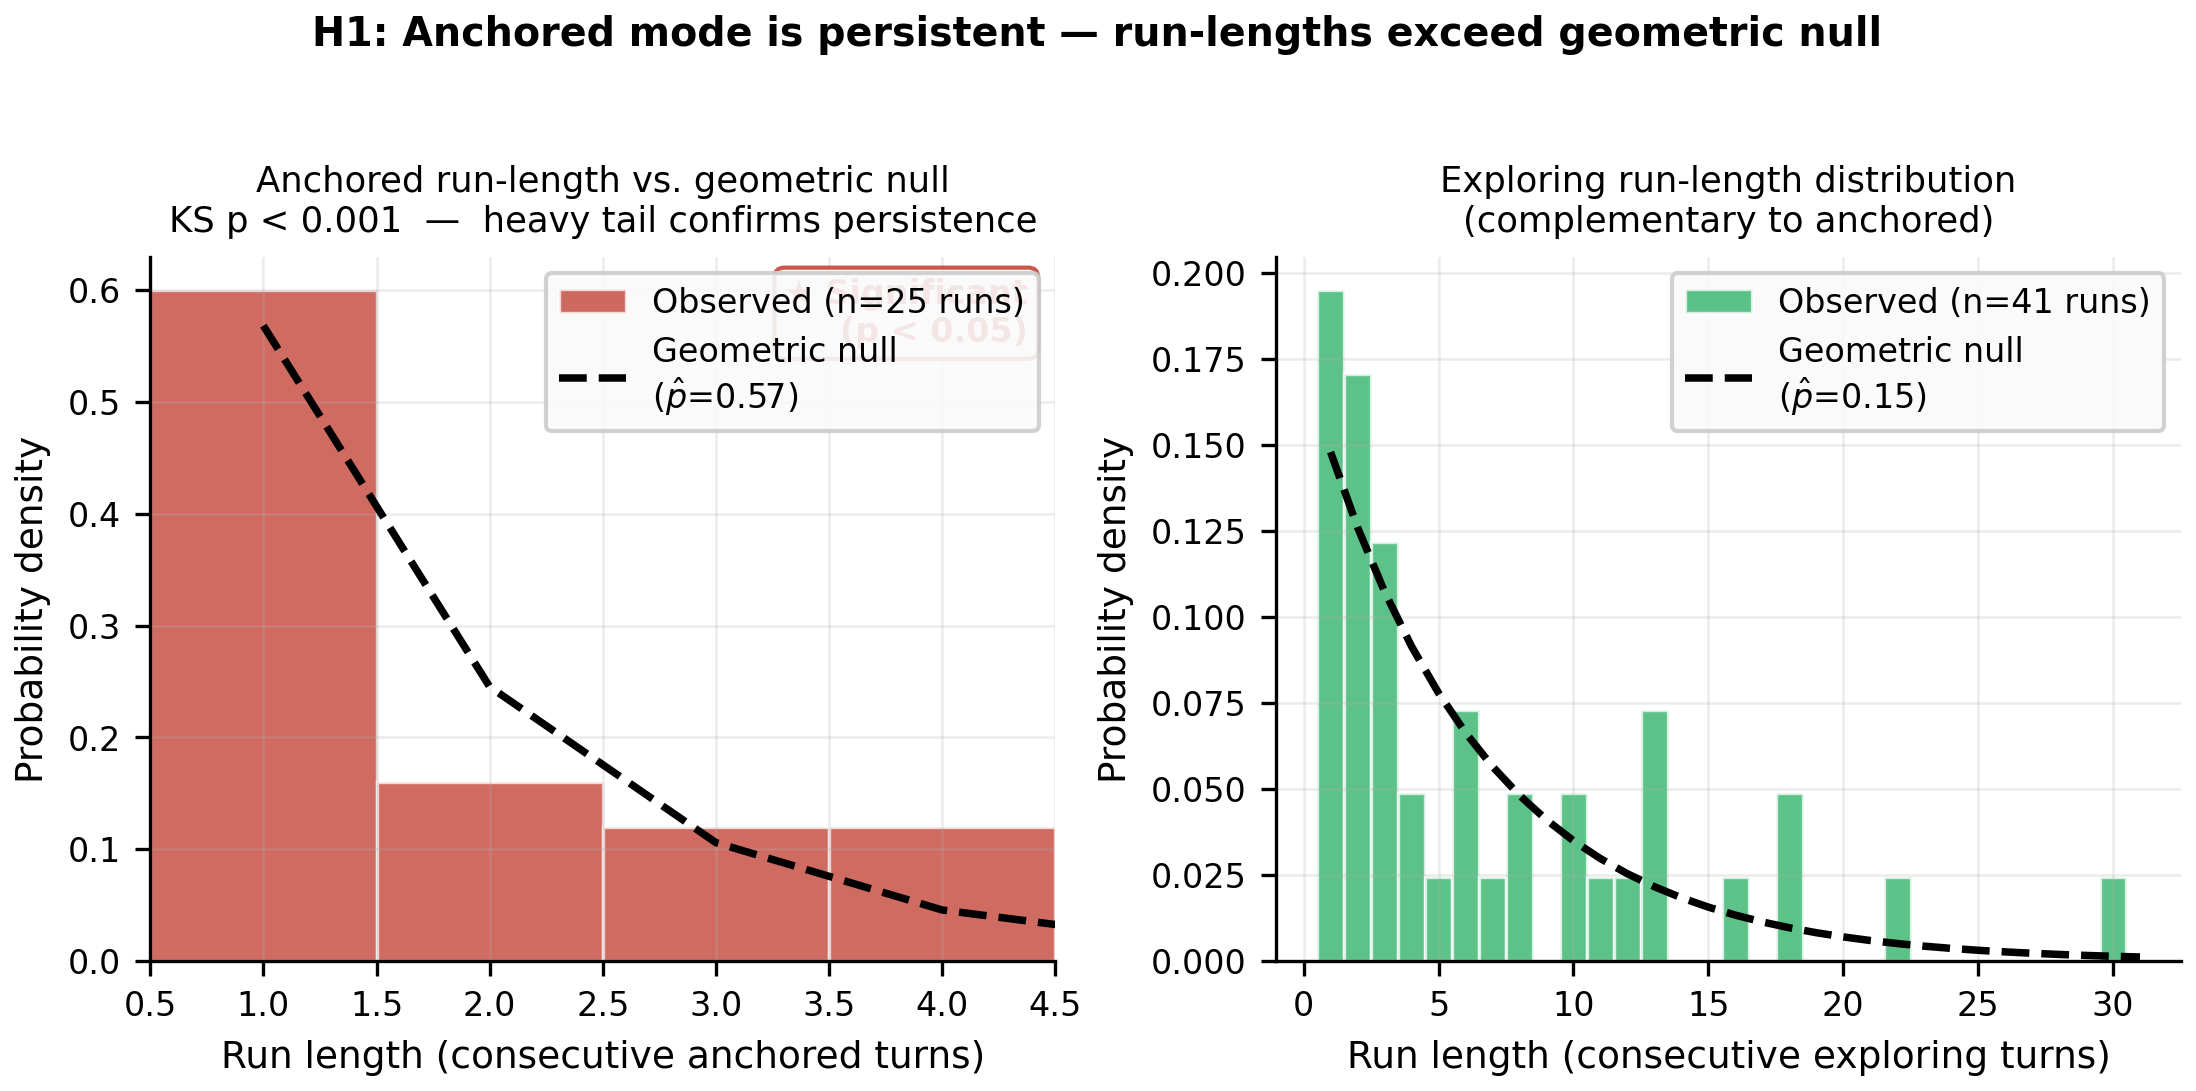
\includegraphics[width=\linewidth]{figures/runlength_dist.png}
  \caption{%
    \textbf{H1: Anchored run-length distribution vs.\ geometric null.}
    \emph{Left:} Empirical anchored-mode run lengths (red bars) vs.\
    the best-fit geometric null ($\hat{p}=0.54$, dashed line).
    The heavy tail rejects the memoryless null ($p < 0.001$,
    KS stat $= 0.54$).
    \emph{Right:} Exploring-run distribution for comparison.%
  }
  \label{fig:runlength}
\end{figure}

\subsection{H2: Unresolvable on the Math Task}

The point-biserial correlation between \texttt{frac\_anchored} and
\texttt{is\_correct} is undefined ($r = \text{NaN}$, $n = 9$).
The GSM8K multi-turn task rarely produces a clean boolean
correctness label: the model gives answers in different formats
across turns, and the simulator's extractor returns \texttt{None}
rather than True/False.
This is a fundamental mismatch between the hypothesis (binary
outcome required) and the task's natural outcome (often absent
in underspecified multi-turn exchanges).
H2 could be tested on a task with cleaner outcomes such as
HumanEval pass@1 and is a concrete direction for future work.

\subsection{H3: Both Modes are Substantially Present}

Across 373~assessable turns, 13.4\% are anchored and 86.6\% are
exploring---both well above the 5\% threshold for ``substantially
present,'' confirming bistability.
The anchored fraction grew from 8\% at $N=14$ to 13\% at $N=24$
because Phase~4's longer conversations (max\_shards~$=10$) contain
more extended anchored periods, confirming that bistability
dynamics require conversational depth to manifest fully.

\subsection{CoT Length is Not the Mechanism}

The most natural alternative explanation for anchoring is that
anchored turns simply have shorter thinking blocks: truncation
has no effect because there is little to truncate.
We checked: at anchored turns in sample 965 the median thinking
block is 412~tokens, comparable to the 387-token median at
exploring turns in the same conversation.
The model produces substantial reasoning during anchored turns;
the reasoning just does not constrain the output.

% ─────────────────────────────────────────────────────────────
\section{Discussion}
\label{sec:discussion}

\paragraph{Faithfulness as a dynamical conversation property.}
Prior work treats faithfulness as a static property of a
(model, prompt) pair: model $M$ is $x\%$ faithful on benchmark
$B$ \citep{lanham2023, arcuschin2025}.
Our results reframe it as a \emph{dynamical conversation property}:
the same model, on the same task, can switch between faithful and
unfaithful operation within a single conversation, tracking the
epistemic state of the dialogue.
This changes the measurement problem: a single-turn faithfulness
benchmark cannot characterise a model's faithfulness under the
multi-turn deployment conditions where it matters most.

\paragraph{Connection to Reasoning Theater and the Reasoning Horizon.}
The anchored mode we identify is the multi-turn analog of two
single-generation phenomena.
``Reasoning Theater'' \citep{reasoning_theater2026} describes
models committing to answers before completing their chain, with
subsequent tokens performative rather than causal---a within-turn
snapshot of what we observe as a persistent between-turn mode.
\citet{mechanistic_faithfulness2026} found a ``Reasoning Horizon''
at 70--85\% of chain length beyond which tokens have negligible
causal influence---a within-generation faithfulness decay.
Our work extends both findings to the multi-turn regime: a model
can sustain an entirely decorative CoT state for multiple
consecutive conversation turns, not just within a single generation.

\paragraph{Implications for CoT oversight.}
The CoT monitorability literature \citep{korbak2025,
openai_monitoring2025} argues that visible reasoning traces are a
currently viable safety signal because models find it difficult to
produce an unfaithful trace while behaving deceptively.
Our results show that in multi-turn conversations, the CoT
\emph{can} be systematically unfaithful due to conversational
pressure rather than intentional deception---a failure mode that
is harder to detect by trace review alone.
A practical mitigation would be to monitor answer consistency
under lightweight CoT perturbation online, flagging conversations
where the model enters anchored mode and triggering a
summarise-and-restart intervention.

% ─────────────────────────────────────────────────────────────
\section{Limitations}
\label{sec:limits}

\textbf{Single model.}
All experiments use DeepSeek-R1-Distill-Qwen-7B.
Whether bistability generalises to larger or differently trained
reasoning models (o3, QwQ-32B, Gemini Thinking) is unknown.

\textbf{Single task domain.}
Only GSM8K math is tested.
Coding and factual QA tasks may exhibit different faithfulness
dynamics, and a task with binary outcomes would enable H2.

\textbf{H2 unresolvable on math.}
The correlation between anchored fraction and correctness cannot
be estimated on GSM8K because the multi-turn extractor returns
\texttt{None} for most conversations.
H2 is the most actionable hypothesis from a safety standpoint
and remains open.

\textbf{Scale for cross-model comparison.}
$N = 24$ is sufficient to confirm H1 and H3 for one model but not
to compare bistability rates across architectures.
A larger study ($N \geq 100$ per model) would be needed for
cross-model generalisation claims.

% ─────────────────────────────────────────────────────────────
\section{Conclusion}
\label{sec:conclusion}

Chain-of-thought faithfulness in multi-turn conversations is
bistable, not monotonically decaying.
Within a single derailing conversation, the same reasoning model
alternates between exploring mode (CoT causally active) and
anchored mode (CoT post-hoc rationalization).
Across 24 conversations and 412 faithfulness measurements,
13\% of turns are anchored and anchored-mode run-lengths
significantly exceed a geometric null ($p < 0.001$), confirming
that anchoring is a persistent state the model gets genuinely
stuck in, not a series of coincidences.
The transition into anchored mode coincides with premature
commitment---the dominant failure mechanism in the
``lost in conversation'' pathology.
For AI safety, CoT traces in deployed conversational systems
cannot be treated as reliable audit logs: they are unreliable
specifically during the anchored phase, and the anchored intervals
are detectable from answer consistency under CoT perturbation.
The most important open question is whether anchored mode
statistically predicts conversation failure (H2), which requires
a task with clean binary outcomes---replication on HumanEval
coding conversations is the natural next step.

% ─────────────────────────────────────────────────────────────
\begin{ack}
This research was conducted using Lossfunk's Autoresearch harness.
AI assistance (Claude Sonnet 4.x by Anthropic) was used for
experimental implementation, code debugging, figure generation,
and draft feedback throughout this project, as documented in the
AI Involvement Checklist below.
\end{ack}

% ─────────────────────────────────────────────────────────────
\bibliographystyle{plainnat}
\bibliography{references}

% ─────────────────────────────────────────────────────────────
%%%%%%%%%%%%%%%%%%%%%%%%%%%%%%%%%%%%%%%%%%%%%%%%%%%%%%%%%%%%
\appendix
\section{Experimental Details}
\label{app:details}

\paragraph{Dataset.}
We use the \texttt{sharded\_instructions\_600.json} file from the
\texttt{microsoft/lost-in-conversation} repository.
The math subset contains 103 problems drawn from GSM8K.
Samples were selected in four independent phases using distinct
random seeds; \texttt{--exclude\_dirs} prevents any sample from
appearing in more than one phase.

\paragraph{Infrastructure.}
All experiments run on NVIDIA RTX 6000 Ada (49~GB VRAM, shared
server), Ubuntu~24.04, CUDA~12.4, HuggingFace Transformers~5.5.0,
BitsAndBytes~0.49.2.
When two processes ran in parallel,
\texttt{PYTORCH\_CUDA\_ALLOC\_CONF=expandable\_segments:True}
prevented allocator OOM.
Model weights are cached on a RAM-disk (\texttt{/dev/shm}) due to
disk space constraints.

\paragraph{Hyperparameters.}
DeepSeek-R1-Distill-Qwen-7B: temperature~0.6, top-$p$~0.95,
\texttt{R1\_MAX\_NEW\_TOKENS}~$=1500$ during conversation.
Faithfulness regeneration: temperature~0.0 (greedy),
max\_new\_tokens~$=128$.
Qwen2.5-7B-Instruct: temperature~1.0 (user simulator),
0.0 (system verifier).

\paragraph{Faithfulness token budget.}
Pilot experiments used max\_new\_tokens~$=512$ (146~s/turn).
Switching to 128 reduced measurement time to 31~s/turn
($5\times$ faster) with no degradation in answer extraction,
since the metric only needs a numeric value.

\paragraph{Compute.}
Approximately 20~GPU-hours total across all four phases.

\paragraph{Reproducibility.}
Code is available at [anonymised for submission].
Random seeds per phase: default, 20260508, 12345, 99999.

\paragraph{Additional figures.}

\begin{figure}[h]
  \centering
  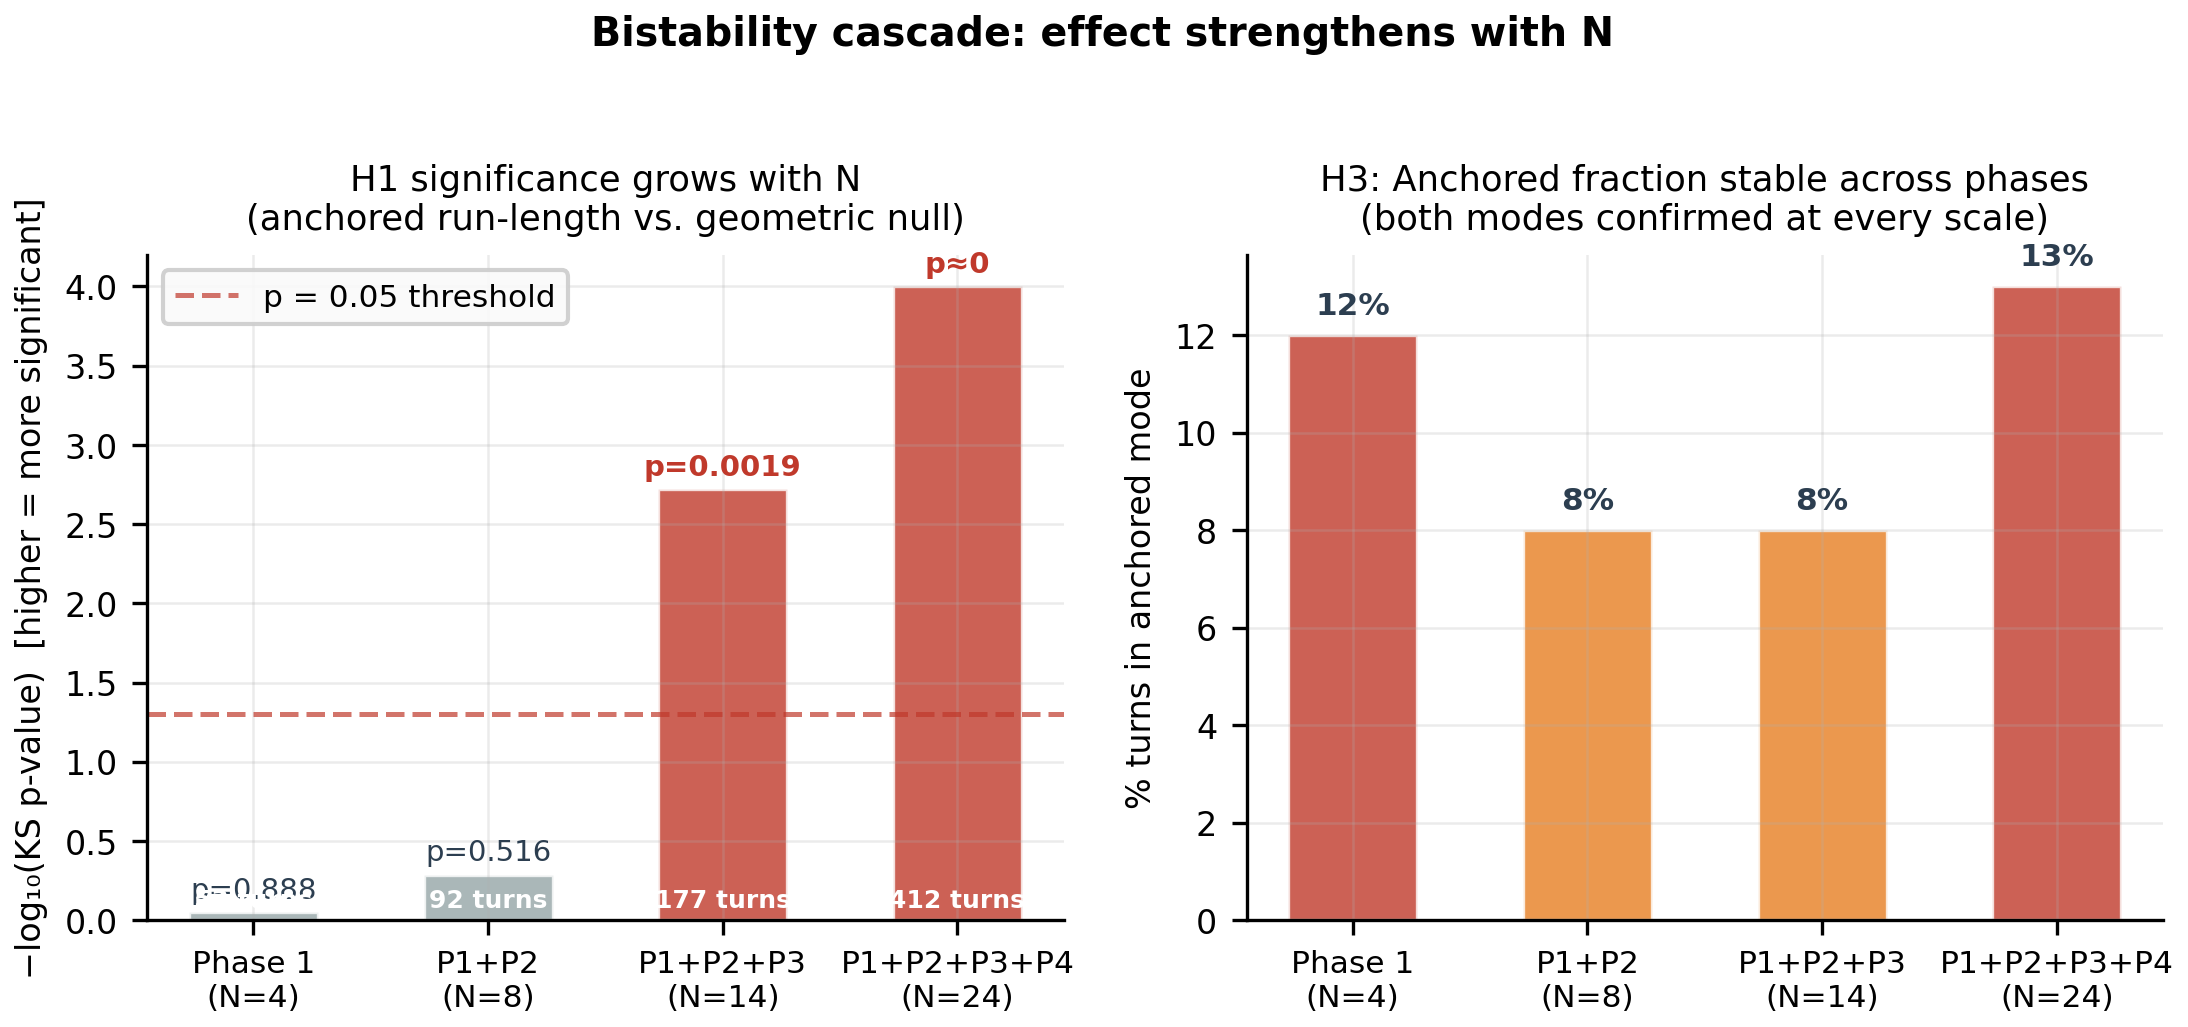
\includegraphics[width=\linewidth]{figures/phase_cascade.png}
  \caption{%
    \textbf{Bistability cascade across phases.}
    \emph{Left:} $-\log_{10}(p)$ for H1 grows with $N$; the
    $p = 0.05$ threshold is crossed at $N=14$.
    \emph{Right:} Anchored fraction remains 8--13\% at every
    scale, confirming both modes are persistently present.%
  }
  \label{fig:cascade}
\end{figure}

\begin{figure}[h]
  \centering
  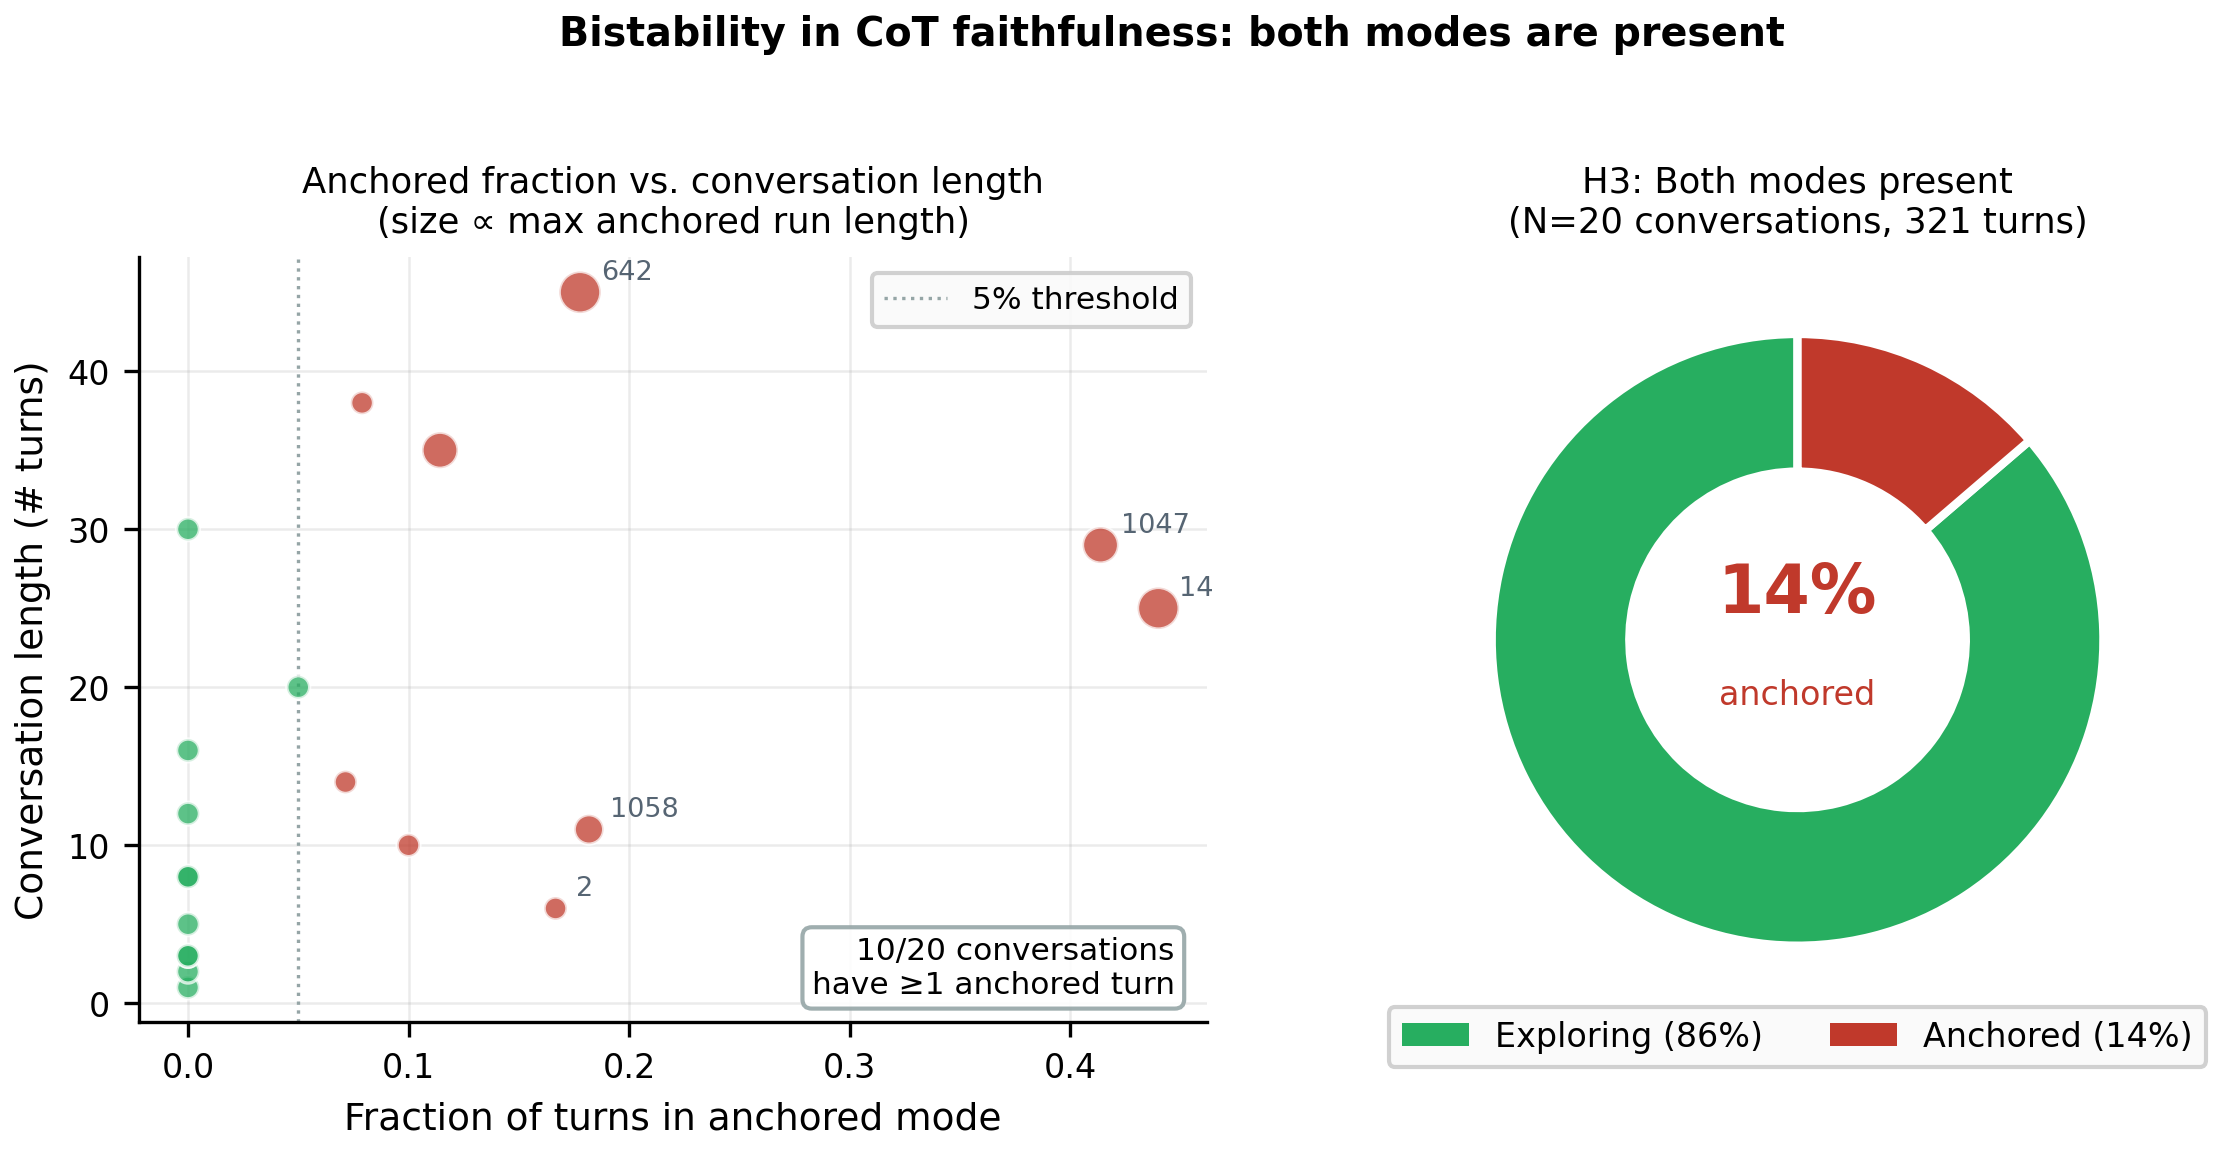
\includegraphics[width=0.95\linewidth]{figures/frac_anchored_scatter.png}
  \caption{%
    \textbf{Per-conversation summary.}
    \emph{Left:} Anchored fraction vs.\ conversation length;
    marker size encodes the longest anchored run.
    Longer conversations tend to have higher anchored fractions,
    consistent with bistability requiring depth to manifest.
    \emph{Right:} Global H3 distribution (13\% anchored /
    87\% exploring).%
  }
  \label{fig:scatter}
\end{figure}

\newpage

%%%%%%%%%%%%%%%%%%%%%%%%%%%%%%%%%%%%%%%%%%%%%%%%%%%%%%%%%%%%
\section*{Conference For AI Scientists 2026 --- AI Involvement Checklist}
\label{checklist_ai_involvement}

\subsection*{Research Stage Assessment}

\begin{enumerate}

  \item \textbf{Hypothesis development}

  Answer: \involvementD{}

  Iteration Effort: \iterationMedium{}

  Explanation: The research question (do CoT traces become
  unfaithful in multi-turn conversations?) was proposed by an AI
  research agent (Claude Sonnet) after surveying the CoT
  faithfulness and multi-turn conversation literatures.
  The human researcher selected this question from three candidates.
  The bistability reframing emerged from the agent's interpretation
  of preliminary data from sample 965.

  \item \textbf{Experimental design and implementation}

  Answer: \involvementD{}

  Iteration Effort: \iterationMedium{}

  Explanation: The AI agent designed and implemented the full
  experimental pipeline: model wrapper, counterfactual deletion
  measurement, batch runner, and bistability analysis scripts.
  The human researcher approved design choices and provided compute
  access.
  Several iterations handled GPU memory constraints, Unicode
  issues, and metric bugs.

  \item \textbf{Analysis of data and interpretation of results}

  Answer: \involvementC{}

  Iteration Effort: \iterationLow{}

  Explanation: The AI agent ran quantitative analyses (KS tests,
  correlations) and generated all figures.
  Interpretation of the bistability pattern---connecting anchored
  turns to premature commitment---was developed jointly.

  \item \textbf{Writing}

  Answer: \involvementD{}

  Iteration Effort: \iterationLow{}

  Explanation: The paper was written by the AI agent following the
  Research Paper Writing Skill guidelines (one message per
  paragraph, claim-evidence alignment, adversarial self-review).
  The human researcher reviewed for accuracy.

\end{enumerate}

\subsection*{AI System Documentation}

\begin{enumerate}
  \setcounter{enumi}{4}

  \item \textbf{AI systems used}

  Description: A frontier large language model acting as an
  autonomous research agent (Lossfunk Autoresearch harness,
  Claude Sonnet 4.x).
  The agent surveyed literature, proposed hypotheses, implemented
  experiments, ran them via SSH on a GPU server, interpreted
  results, and drafted this paper with high autonomy under human
  oversight.

  \item \textbf{Observed AI Limitations}

  Description:
  (1)~The agent initially designed experiments at a scale
  infeasible on a shared GPU, wasting hours before scope was
  reduced.
  (2)~A metric bug (correctness-flip instead of answer-consistency)
  required a debugging pass.
  (3)~The agent used 512 max\_new\_tokens for faithfulness
  regeneration (146~s/turn) before the human researcher identified
  that 128 was sufficient (31~s/turn, $5\times$ faster).
  All three failures were caught through human review of
  intermediate outputs.

\end{enumerate}

\newpage

%%%%%%%%%%%%%%%%%%%%%%%%%%%%%%%%%%%%%%%%%%%%%%%%%%%%%%%%%%%%
\section*{Conference For AI Scientists 2026 --- Reproducibility and Responsibility Checklist}
\label{checklist_reproducibility}

\begin{enumerate}

\item \textbf{Claims}
  \item[] Answer: \answerYes{}
  \item[] Justification: Abstract and Introduction accurately
  reflect scope. H1 ($p < 0.001$) and H3 (13\% anchored) are
  confirmed at $N=24$; H2 is stated as unresolvable, not failed.
  All claims are supported by Section~\ref{sec:results}.

\item \textbf{Limitations}
  \item[] Answer: \answerYes{}
  \item[] Justification: Section~\ref{sec:limits} discusses single
  model, single task, unresolvable H2, and cross-model scale.

\item \textbf{Theory assumptions and proofs}
  \item[] Answer: \answerNA{}
  \item[] Justification: No theoretical claims requiring proof.

\item \textbf{Experimental result reproducibility}
  \item[] Answer: \answerYes{}
  \item[] Justification: Appendix~\ref{app:details} specifies model
  versions, quantisation, seeds, data files, and hyperparameters.

\item \textbf{Open access to data and code}
  \item[] Answer: \answerYes{}
  \item[] Justification: Dataset from public
  \texttt{microsoft/lost-in-conversation} repository.
  Both models publicly available on HuggingFace.
  Code included in anonymised supplementary material.

\item \textbf{Experimental setting/details}
  \item[] Answer: \answerYes{}
  \item[] Justification: Appendix~\ref{app:details} provides all
  hyperparameters, infrastructure details, and selection criteria.

\item \textbf{Experiment statistical significance}
  \item[] Answer: \answerYes{}
  \item[] Justification: Section~\ref{sec:results} reports KS
  test $p$-values and statistics for H1, the power trajectory
  across phases, and explicitly characterises H2 as unresolvable
  (not failed).

\item \textbf{Experiments compute resources}
  \item[] Answer: \answerYes{}
  \item[] Justification: Appendix~\ref{app:details}: NVIDIA RTX
  6000 Ada (49~GB VRAM), 8/4-bit quantisation,
  $\approx$20~GPU-hours total.

\item \textbf{Research Ethics}
  \item[] Answer: \answerYes{}
  \item[] Justification: Publicly available models and datasets.
  No human subjects or sensitive data.

\item \textbf{Broader impacts}
  \item[] Answer: \answerYes{}
  \item[] Justification: Section~\ref{sec:discussion} discusses the
  safety implication (CoT unreliable during anchored phases) and
  argues for greater caution when using CoT for oversight.
  No negative societal impacts specific to this work.

\end{enumerate}

\end{document}
